\documentclass[10pt,UTF8]{book} %% ctexart

\title{\textbf{离散数学}讲义}
\author{钱锋\thanks{Email: strik0r\_qf@mail.nwpu.edu.cn}}

\usepackage{ctex}
\usepackage{graphicx}
\usepackage[toc]{multitoc}
\usepackage{amsthm, amssymb, amsmath, mathrsfs, mhchem}
\usepackage{tikz,circuitikz}
\usetikzlibrary{decorations.markings, angles, quotes}
\usepackage{pgfplots}
\usepackage{subcaption}
\usepackage{tikz-3dplot}
\usepackage{extpfeil}
\usepackage{diagbox}
\usepackage{float}
\usepackage{hyperref}
\hypersetup{hidelinks,
    colorlinks = true,
    allcolors = black,
    pdfstartview = Fit,
    breaklinks = true}
\usepackage{caption}
\usepackage{enumitem}
\usepackage{siunitx}
% 定义带圆圈的数字命令
\newcommand{\circled}[1]{\textcircled{\small #1}}

\usepackage{fancyhdr} % 用于自定义页眉页脚


% 设置页眉页脚样式
\fancypagestyle{plain}{%
    \fancyhf{} % 清空页眉页脚
    \fancyhead[RO,LE]{·\thepage·} % 页眉显示页码, RO表示奇数页右侧, LE表示偶数页左侧
    \fancyhead[LO]{\nouppercase{\rightmark}} % 页眉显示小节标题, LO表示奇数页左侧
    \fancyhead[RE]{\nouppercase{\leftmark}} % 页眉显示章节标题, RE表示偶数页右侧
    \renewcommand{\headrulewidth}{0.4pt} % 设置页眉横线的宽度
    \renewcommand{\footrulewidth}{0pt} % 取消页脚横线
}

\renewcommand{\headrule}{\hrule width\textwidth height\headrulewidth\vskip-\headrulewidth}

% % 取消奇偶页的页眉偏移
% \fancyhfoffset[RO,LE]{0pt}

% % 取消奇偶页的页眉偏移
% \fancyhfoffset[RO,LE]{0pt}

% 定义取消页眉的命令
\newcommand{\cancelheader}{%
    \fancyhead{} % 清空页眉
    \renewcommand{\headrulewidth}{0pt} % 取消页眉横线
    \renewcommand{\footrulewidth}{0pt} % 设置页脚横线的宽度
}

\renewcommand{\chaptermark}[1]{\markboth{第 \thechapter 章 \hspace{1em} #1}{}}
\renewcommand{\sectionmark}[1]{\markright{\thesection \, #1}}

\usepackage{tasks}
\usepackage{titlesec} % 定义标题样式

% 设置 chapter 标题样式
\titleformat{\chapter}[hang]{\centering\heiti\Large\bfseries}{专题\,\thechapter}{1em}{}

% 定义 section 标题格式
\titleformat{\section}[hang]{\heiti\centering\large\bfseries}{\thesection}{1em}{}

% 定义 subsection 标题格式
\titleformat{\subsection}[hang]{\heiti\bfseries}{\textbf{\thesubsection}}{1em}{}

% 定义 subsubsection 标题格式
\setcounter{secnumdepth}{3}
\renewcommand\thesubsubsection{\arabic{subsubsection}.}
\titleformat{\subsubsection}[hang]{\kaishu}{\quad\quad\thesubsubsection\,\,}{0em}{}

% 设置页边距和对齐
% \usepackage[
%     paperwidth=185mm,
%     paperheight=260mm,
%     top=35mm,
%     bottom=25mm,
%     left=18mm,
%     right=18mm,
%     footskip=15mm % 通过这里的值来调整页脚与正文内容的垂直距离
% ]{geometry}

\usepackage[
    paperwidth=210mm,
    paperheight=297mm,
    top=40mm,
    bottom=31.8mm,
    left=25.4mm,
    right=25.4mm,
    footskip=15mm % 通过这里的值来调整页脚与正文内容的垂直距离
]{geometry}

% \usepackage[
%     paperwidth=195mm,
%     paperheight=270mm,
%     top=40mm,
%     bottom=25mm,
%     left=23.5mm,
%     right=23.5mm,
%     footskip=15mm % 通过这里的值来调整页脚与正文内容的垂直距离
% ]{geometry}
\usepackage{mdframed}
\mdfsetup{
  linewidth=0.4pt,
  frametitlebackgroundcolor=white, % 或者 transparent
  frametitlefont=\heiti\bfseries,
  frametitleaboveskip=10pt,
  frametitlebelowskip=5pt,
  frametitlealignment=\raggedright % 新增此行
}
\usepackage{fontspec}
% 设置 Menlo 字体
\setmonofont{Menlo}
\usepackage{fancyvrb}
\usepackage{xcolor}
\usepackage{listings}

% \definecolor{string}{HTML}{067D17}
% \definecolor{comment}{HTML}{8C8C8C}
% \definecolor{keyword}{HTML}{0033B3}
% \definecolor{class_field}{HTML}{871094}

\lstset{breaklines}
%这条命令可以让LaTeX自动将长的代码行换行排版
\lstset{extendedchars=false}
%这一条命令可以解决代码跨页时,章节标题,页眉等汉字不显示的问题
\lstset{escapeinside={(*}{*)}}

\lstset{
    basicstyle=\small\ttfamily\heiti,
    numbers=left,
    numberstyle=\scriptsize\fontspec{Menlo}, % 使用 Menlo 字体
    stepnumber=1,
    numbersep=8pt,
    frame=leftline,
    xleftmargin=2em, % 调整代码块的左边界
    framexleftmargin=0pt, % 调整边框的位置
    breaklines=true,
    % postbreak=\mbox{\textcolor{red}{$\hookrightarrow$}\space},
    % keywordstyle=\bfseries\color{keyword},          % keyword style
    % commentstyle=\heiti\color{comment},       % comment style
    % stringstyle=\color[HTML]{067D17},
    showstringspaces=false,
    % string literal style
    % escapeinside={\%*}{*)},            % if you want to add LaTeX within your code
    % morekeywords={}               % if you want to add more keywords to the set
}

\usepackage{smartdiagram}
\usepackage{subcaption}

\begin{document}

\newtheoremstyle{mytheoremstyle}
    {1.5ex}                                         % Space above
    {1.5ex}                                         % Space below
    {}                                              % Font for body
    {}                                              % Indent amount
    {\bfseries}                                     % Font for head
    {}                                              % Punctuation after head
    {0.5em plus 0.2em minus 0.1em}                  % Space after head
    {\thmname{#1}\thmnumber{ #2}.\thmnote{ (#3).}}

\theoremstyle{mytheoremstyle}
\newtheorem{definition}{定义}[section]
\newtheorem{example}{例}[section]
\newtheorem{exercise}{习题}[chapter]
\newtheorem{code}{程序清单}[section]
\newtheorem*{result}{运行结果}

\newtheoremstyle{my2theoremstyle}
    {1.5ex}                                         % Space above
    {1.5ex}                                         % Space below
    {\kaishu}                                              % Font for body
    {}                                              % Indent amount
    {\bfseries}                                     % Font for head
    {}                                              % Punctuation after head
    {0.5em plus 0.2em minus 0.1em}                  % Space after head
    {\thmname{#1}\thmnumber{ #2}.\thmnote{ (#3).}}

\theoremstyle{my2theoremstyle}
\newtheorem{thm}{定理}[section]
\newtheorem{law}{定律}[section]
\newtheorem{educt}{推论}
\newtheorem{prop}{命题}
\newtheorem{lemma}{引理}
\newtheorem{axiom}{公理}
\newtheorem{property}{性质}

\newtheoremstyle{my4theoremstyle}
    {1.5ex}                                         % Space above
    {1.5ex}                                         % Space below
    {}                                              % Font for body
    {}                                              % Indent amount
    {\bfseries}                                     % Font for head
    {}                                              % Punctuation after head
    {0.5em plus 0.2em minus 0.1em}                  % Space after head
    {\thmname{#1}.}

\theoremstyle{my4theoremstyle} \newtheorem*{sol}{解}

\newtheoremstyle{my3theoremstyle}
    {1.5ex}                                         % Space above
    {1.5ex}                                         % Space below
    {}                                              % Font for body
    {}                                              % Indent amount
    {\kaishu}                                       % Font for head
    {}                                              % Punctuation after head
    {0.5em plus 0.2em minus 0.1em}                  % Space after head
    {\thmname{#1}\thmnumber{ #2}.\thmnote{ (#3).}}

\theoremstyle{my3theoremstyle} \newtheorem*{remark}{注}
\newtheorem*{cmt}{评注}

\begin{titlepage}
    \thispagestyle{empty}
    \centering
        \vspace*{2cm}
        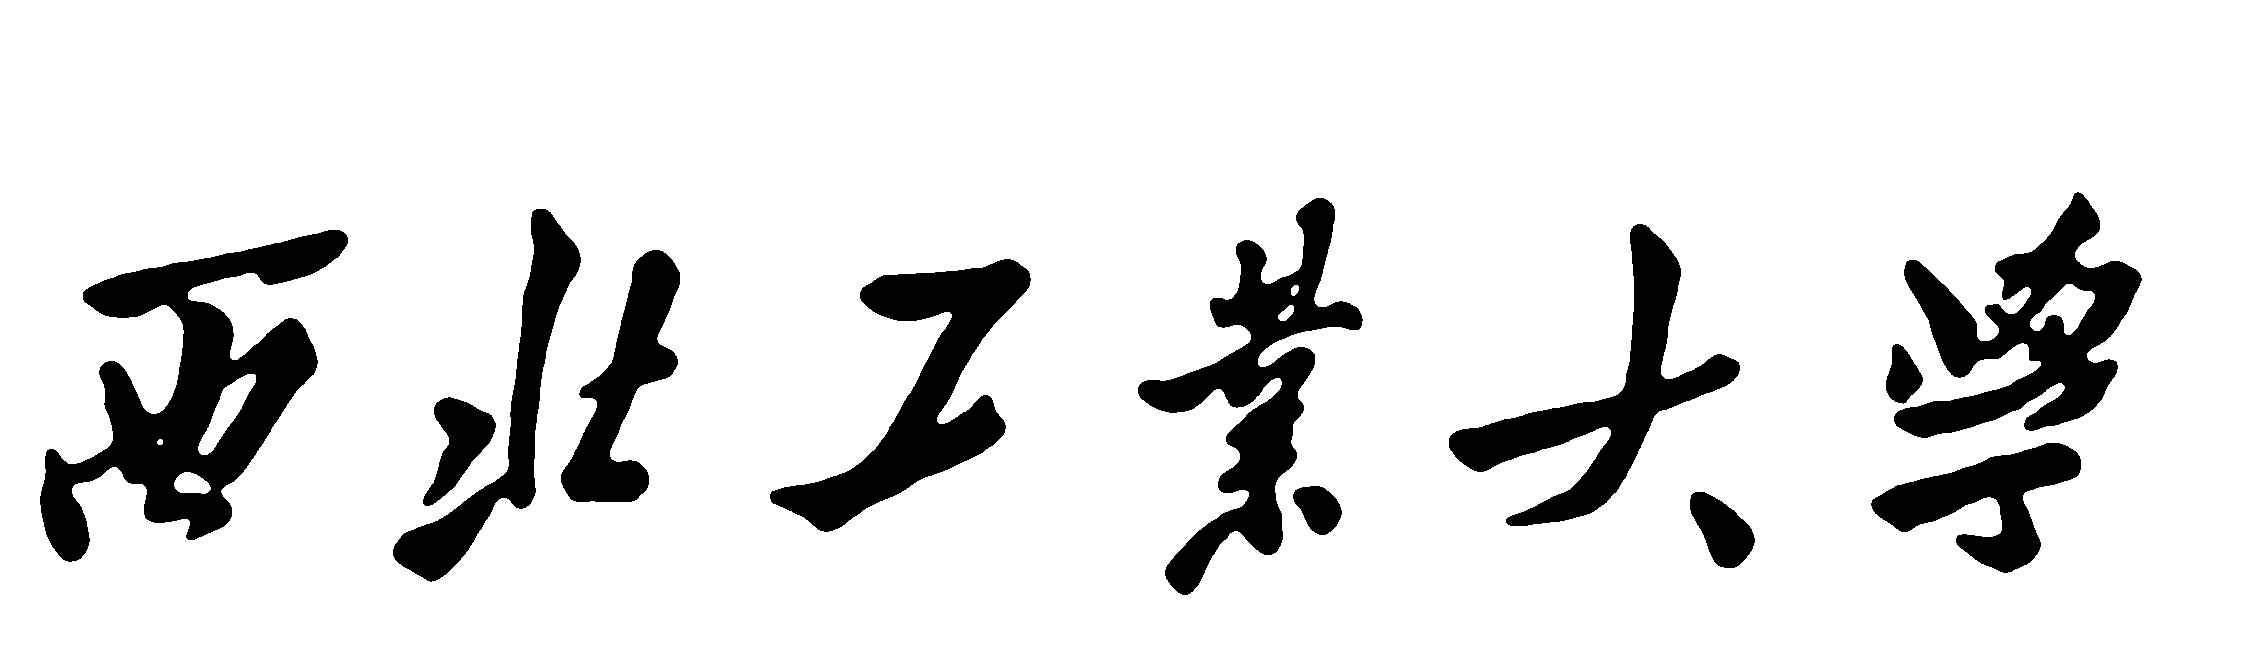
\includegraphics[width=0.5\textwidth]{pic/npu_2.png}\par
        \vspace{1em}
        
\includegraphics[width=0.5\textwidth]{pic/npu_1.png}\par
    \vspace{2em}
        \begin{center}
            \Huge \heiti \textbf{离散数学习题集}

            Problem Set of Discrete Mathematics
        \end{center}
        \vspace{3cm}
        \begin{center}
        \songti
        \renewcommand\arraystretch{1.5}
	\begin{tabular}{p{2cm} c c}
    {姓\,\,\,\,\,\,\,\,\,\,\,\,名:} & \multicolumn{2}{c}{钱 \quad\quad 锋}\\
    \cline{2-3}
    % {编\,\,\,\,\,\,\,\,\,\,\,\,号:} & \multicolumn{2}{c}{13} \\
    % \cline{2-3}
    {班\,\,\,\,\,\,\,\,\,\,\,\,级:} & \multicolumn{2}{c}{14012203} \\
    \cline{2-3}
    {学\,\,\,\,\,\,\,\,\,\,\,\,号:} & \multicolumn{2}{c}{2022303324}\\
    \cline{2-3}
    {邮\,\,\,\,\,\,\,\,\,\,\,\,箱:} & \multicolumn{2}{c}{strik0r.qf@gmail.com}\\
    \cline{2-3}
    {日\,\,\,\,\,\,\,\,\,\,\,\,期:} & \multicolumn{2}{c}{\today}\\
    \cline{2-3}
	\end{tabular}
    \end{center}
\end{titlepage}

\frontmatter
\newpage
\pagestyle{plain}
\makeatother

% \input{丛书前言.tex}

% \chapter{课程概述}
% \thispagestyle{empty}

% \quad\quad 离散数学是以研究离散量的结构和相互间的关系为主要目标的数学分支,
% 是综合了分析学、代数学、集合论、数理逻辑、关系论、函数论、图论与组合数学的综合性学科.

\newpage
\thispagestyle{empty}

% 设置目录页的页码格式
\pagenumbering{roman} % 切换回罗马数字页码
\addtocontents{toc}{\protect\thispagestyle{empty}}
\pagestyle{plain}
{\tableofcontents}
\newpage
\thispagestyle{empty}
\cleardoublepage % 确保正文从奇数页开始


% 设置章节标题页的页眉和页脚为空白页样式
\makeatletter
\let\ps@plain\ps@empty
\makeatother

\mainmatter

\chapter{命题逻辑}

\section{第一讲 (2024.2.27)}

\begin{exercise}
    设 $p$ 为 $2$ 是素数, $q$ 为 $3$ 是素数, $r$ 为 $\sqrt{2}$ 为有理数.
    下列符合命题中哪一个是假命题?
    \begin{itemize}[itemsep=0pt]
        \item $(p \vee q) \longrightarrow r$. 我们先判断一下 $p,q,r$ 的真值,
        显然 $p=1,q=1,r=0$, 于是 $(p \vee q) = 1$, 根据蕴含式的真值规则,
        前件为真, 后件为假, 该命题为假命题.
        \item $r \longrightarrow (p \vee q)$. 根据蕴含式的真值规则, 当前件为假时
        无论后件为真命题还是假命题, 蕴含式为真, 所以由 $r=0$ 知这是一个真命题.
        \item $(p \wedge q) \longrightarrow p$. 根据合取式的真值表, $(p \wedge q)=1$,
        前件为真, 后件为真, 这是一个真命题.
        \item $(r \vee p) \longleftrightarrow q$. 根据 $p,q,r$ 的真值可知,
        $(r \vee p)=1, q=1$, 于是根据等价式的真值规则, 这是一个真命题.
    \end{itemize} 
\end{exercise}

\begin{exercise}
    判断下列语句是否为命题, 如果是命题, 请指出其真值.
    \begin{itemize}[itemsep=0pt]
        \item \textbf{中国是一个人口众多的国家}. 这是一个陈述句, 并且在特定的语境下能够判断其陈述内容
        的真假, 例如在上下文中有关于 “人口众多” 的定义和明确的判定标准时, 这个陈述句就是可以
        明确判定真假的, 因此它是一个命题. 除此之外, 根据常识可知, 中国是目前人口最多的国家,
        当然称得上是人口众多 (毕竟都已经是最多的那一个了, 再算不上众多的话说明众多的定义需要
        修正一下了), 所以这是一个真命题.
        \item \textbf{存在最大的素数}. 这是一个典型的数学命题, 根据素数的有关研究结果我们
        知道它是一个假命题.
        \item \textbf{这座楼可真高啊}. 这是一个感叹句, 因此它不是一个命题. 如果改成 “这座楼有
        超过 50 层” 的话就是一个命题了.
        \item \textbf{请你跟我走}. 这是一个祈使句, 它不是命题.
        \item \textbf{火星上也有人}. 这是一个陈述句, 并且是能够判断它的真假的 —— 有人, 或者没有人,
        必居其一且只居其一, 所以这是一个命题. 虽然目前我们的科学研究并不能严格的说明火星上
        是否有人存在, 但是按照目前的主流观点来看, 火星上是没有人的, 所以我们说这个命题
        在这意义下是一个假命题.
    \end{itemize}
\end{exercise}

\begin{exercise}
    将下列命题符号化.
    \begin{itemize}[itemsep=0pt]
        \item “虽然交通堵塞, 但是老王还是准时到达火车站”. 设 $p$ 为交通拥堵,
        设 $q$ 为老王准时到达火车站. 显然这里的转折关系是表示这两件事情同时发生的,
        因此应该取它们二者的合取命题, 即 $p \wedge q$.
        \item “张小宝是三好生, 它是北京人或河北人”. 设 $p$ 为张小宝是三好生,
        $q$ 表示张小宝是北京人, $r$ 表示他来自河北. 这里的逗号显然表示了并列关系,
        因此应该取 $p \wedge (q \vee r)$.
        \item “除非天下雨, 否则我骑车上班”. 这句话的意思就是说, 如果天不下雨那么我就要
        骑车去上班, 设 $p$ 表示雨天, $q$ 表示我骑车去上班, 那么表示为
        $(\lnot p) \longrightarrow q$.
    \end{itemize}
\end{exercise}

\begin{exercise}
    设命题 $p,q$ 的真值为 F, 命题 $r,s$ 的真值为 T, 求公式 $(p \longleftrightarrow r)
    \wedge ((\lnot q) \vee s)$ 的真值.
    \begin{sol}
        直接代入 $p,q,r,s$ 的真值, 得到
        \[ (0 \leftrightarrow 1)\wedge((\lnot 0) \vee 1), \]
        根据等价式和逻辑或的真值规则, 它实际上就是
        \[ 0 \wedge 1, \]
        根据逻辑与的运算规则, 原命题的真值应该为 F.
    \end{sol}
\end{exercise}

\section{第二讲 (2024.2.29)}

\begin{exercise}
    证明下列等价关系:
    \begin{itemize}[itemsep=0pt]
        \item $p \to (q \to p) \equiv \lnot p \to (p \to \lnot q)$.
        \begin{proof}
            \begin{table}[H]
                \centering
                \caption{$p \to (q \to p)$ 和 $\lnot p \to (p \to \lnot q)$ 的真值表}
                \begin{tabular}{cccccccc}
                    \hline
                    $p$ & $q$ & $q \to p$ & $p \to (q \to p)$ & $\lnot p$ & $\lnot q$ & $p \to \lnot q$ & $\lnot p \to (p \to \lnot q)$ \\
                    \hline
                    0 & 0 & 1 & 1 & 1 & 1 & 1 & 1 \\
                    0 & 1 & 0 & 1 & 1 & 0 & 1 & 1 \\
                    1 & 0 & 1 & 1 & 0 & 1 & 1 & 1 \\
                    1 & 1 & 1 & 1 & 0 & 0 & 0 & 1 \\
                    \hline
                \end{tabular}
            \end{table}
            容易验证它们所在的两列是完全相同的, 因此它们逻辑等价.
            在下面几例中不再赘述, 仅列出真值表.
        \end{proof}
        \item $(p \to q)\wedge(r \to q) \equiv ((p \vee r) \to q)$.
        \begin{table}[H]
            \centering
            \begin{tabular}{cccccccc}
                \hline
                $p$ & $q$ & $r$ & $p \to q$ & $r \to q$ & $(p \to q) \wedge (r \to q)$ & $p \vee r$ & $(p \vee r) \to q$ \\ 
                \hline
                0 & 0 & 0 & 1 & 1 & 1 & 0 & 1 \\ 
                0 & 0 & 1 & 1 & 0 & 0 & 1 & 0 \\ 
                0 & 1 & 0 & 1 & 1 & 1 & 0 & 1 \\
                0 & 1 & 1 & 1 & 1 & 1 & 1 & 1 \\
                1 & 0 & 0 & 0 & 1 & 0 & 1 & 0 \\
                1 & 0 & 1 & 0 & 0 & 0 & 1 & 0 \\
                1 & 1 & 0 & 1 & 1 & 1 & 1 & 1 \\
                1 & 1 & 1 & 1 & 1 & 1 & 1 & 1 \\
                \hline 
            \end{tabular}
        \end{table}
        \item $\lnot(p \leftrightarrow q) \equiv (p \vee q) \wedge (\lnot(p \wedge q)) \equiv (p \wedge \lnot q)\vee(\lnot p \wedge q)$.
        \begin{table}[H]
            \centering
            \begin{tabular}{ccccc}
                \hline
                $p$ & $q$ & $\lnot(p \leftrightarrow q)$ & $(p \vee q) \wedge (\lnot p \wedge q)$ & $(p \wedge \lnot q) \vee (\lnot p) \wedge q$ \\
                \hline 
                0 & 0 & 0 & 0 & 0 \\
                0 & 0 & 1 & 1 & 1 \\
                1 & 0 & 1 & 1 & 1 \\
                1 & 1 & 0 & 0 & 0 \\
                \hline
            \end{tabular}
        \end{table}
        \item $\lnot (p \to q) \equiv p \wedge \lnot q$.
        \begin{proof}
            这是显然成立的, 因为 $p \to q \equiv \lnot p \vee q$, 我们只需要两边取反即可.
        \end{proof}
    \end{itemize}
\end{exercise}

\begin{exercise}
    求出下列公式的最简等价式:
    \begin{itemize}[itemsep=0pt]
        \item $((p \leftrightarrow q) \leftrightarrow (\lnot q \to \lnot p))\wedge r$.
        \begin{sol}
            我们采用布尔代数的记号来简化我们的书写和计算, 我们\textbf{约定 $a+b$ 表示 $a \vee b$,
            $ab = a \cdot b$ 表示 $a \wedge b$, $\bar a$ 表示 $\lnot a$}. 由于布尔代数
            和命题逻辑都是同一个更一般的代数结构的具体形式, 因此这种符号的替代和运算的相互转换,
            以及布尔恒等式和逻辑等价式的相互对应是显然成立的. 这样做的好处是, 在求复合命题的否定
            的时候, 可以利用上划线来减少括号的嵌套层数, 在视觉上让公式更加紧凑, 提高公式的可读性. 此外, 关于 $+$
            和 $\cdot$ 的有关运算律是我们所熟识的, 唯一不同的是在布尔代数中逻辑加对逻辑乘依然
            具有分配性, 即 $a + bc = (a+b)(a+c)$.

            由于布尔代数中并没有定义与 $\to$ 和 $\leftrightarrow$ 相对应的基本运算,
            所以我们利用 $p \to q \equiv \lnot p \vee q$ 和
            $p \leftrightarrow q \equiv (p \wedge q)\vee(\lnot p \wedge q)$
            得到两个能表达相同含义的布尔表达式:
            \[ \bar p + q, \quad pq+\bar p \bar q. \]

            现在考虑对原命题公式进行化简, 按照先前的结论, $p \leftrightarrow q$ 对应
            $pq+\bar p \bar q$, 同理, $\lnot q \to \lnot p$ 对应
            $q + \bar p$.
            所以 $(p \leftrightarrow q) \leftrightarrow (\lnot q \to \lnot p)$ 
            对应的布尔表达式为
            \[ (pq + \bar p \bar q)(q + \bar p) + \left(\overline{pq + \bar p \bar q}
            \cdot \overline{q + \bar p}\right). \]
            我们先考虑 $(pq + \bar p \bar q)(q + \bar p)$,
            根据相关的布尔恒等式,
            \[ (pq + \bar p \bar q)(q + \bar p) 
            = pq(q + \bar p) + \bar p \bar q (q + \bar p)
            = pqq + pq\bar p + \bar p \bar q q + \bar p \bar q \bar p 
            = pq + \bar p \bar q. \]
            而
            \[ \overline{pq + \bar p \bar q}
            = \overline{pq} \cdot \overline{\bar p \bar q}
            = (\bar p + \bar q) (p + q)
            =(\bar p + \bar q)p + (\bar p + \bar q) q 
            = \bar p p + \bar q p + \bar p q + \bar q q 
            = \bar p(p+q), \]
            \[ \overline{q + \bar p} = \bar q p, \]
            因此 \[ \overline{pq + \bar p \bar q}
            \cdot \overline{q + \bar p} = \bar p (p+q) \bar q p = 0. \]
            这就是说,
            \[ (pq + \bar p \bar q)(q + \bar p) + \left(\overline{pq + \bar p \bar q}
            \cdot \overline{q + \bar p}\right) = pq + \bar p \bar q. \]
            于是原命题对应的布尔表达式为
            \[ pqr + \bar p \bar q r. \]
            于是原命题的最简等价式为 $(p \leftrightarrow q) \wedge r$.
        \end{sol}

        \item $p \vee \lnot p \vee (q \wedge \lnot q)$.
        \begin{sol}
            容易得到 $p + \bar p + (q \bar q) = 1 + 0 = 1$,
            于是原命题的最简等价式为 T.
        \end{sol}

        \item $(p \wedge (q \wedge s)) \vee (\lnot p \wedge (q \wedge s))$.
        \begin{sol}
            容易得到 $pqs + \bar p qs = (p + \bar p)qs = qs$.
            于是原命题的最简等价式为 $q \wedge s$.
        \end{sol}
    \end{itemize}
\end{exercise}

\begin{exercise}
    证明下列蕴含式.
    \begin{itemize}[itemsep=0pt]
        \item $p \wedge q \Longrightarrow (p \to q)$.
        \begin{proof}
            只需证明 $p \wedge q \to (p \to q)$
            是永真式即可. 它
            所对应的布尔表达式为 $\overline{pq} + (\bar p + \bar q)$.
            \[ \overline{pq} + (\bar p + \bar q)
            = \bar p + \bar q + \bar p + q
            = \bar p + \bar q + q = \bar p + 1 = 1. \]
            于是上述蕴含式得证.
        \end{proof}
        \item $p \Longrightarrow (q \to p)$.
        \begin{proof}
            $\lnot p + \left( \bar q + p \right) = \bar p + \bar q + p
            = \bar q + 1 = 1$.
        \end{proof}
        \item $(p \to (q \to r)) \Longrightarrow (p \to q) \to (p \to r)$.
        \begin{table}[H]
            \centering
            \begin{tabular}{cccccc}
                \hline
                $p$ & $q$ & $r$ & $p \to (q \to r)$ & $(p \to q) \to (p \to r)$ & $(p \to (q \to r)) \rightarrow (p \to q) \to (p \to r)$ \\
                \hline 
                0 & 0 & 0 & 1 & 1 & 1 \\
                0 & 0 & 1 & 1 & 1 & 1 \\
                0 & 1 & 0 & 1 & 1 & 1 \\
                0 & 1 & 1 & 1 & 1 & 1 \\
                1 & 0 & 0 & 1 & 1 & 1 \\
                1 & 0 & 1 & 1 & 1 & 1 \\
                1 & 1 & 0 & 0 & 0 & 1 \\
                1 & 1 & 1 & 1 & 1 & 1 \\
                \hline
            \end{tabular}
        \end{table}
    \end{itemize}
\end{exercise}

\section{第二周}

\begin{example}
    求下列各式的主析取范式和主合取范式.
    \begin{itemize}[itemsep=0pt]
        \item $(\lnot p \vee \lnot q) \to (p \leftrightarrow \lnot q)$.
        \begin{sol}
            原命题对应的布尔表达式为 $\overline{\bar p \bar q} + \left(
                p\bar q + \bar p q
            \right)$. 根据 De Morgan 定律, 我们有
            \[ p+q + p \bar q + \bar p q \]
            补充变元,
            \[ p(q +\bar q) + (p + \bar p)q + p \bar q + \bar p q = p\bar q + \bar pq + pq \]
            于是主析取范式为 $m_1 \vee m_2 \vee m_3$, 主合取范式为 $M_0$.
        \end{sol}
        \item $p \vee (\lnot p \to (q \vee (\lnot q \to r)))$.
        \begin{sol}
            原命题对应的布尔表达式为 $p+p+(q + q + r)$. 所以
            \[ p(q + \bar q)(r + \bar r) + (p + \bar p)q(r+ \bar r) + (p +\bar p)(q + \bar q)r =
            pqr + pq \bar r + p \bar q r + p \bar q \bar r + \bar p qr + \bar p q \bar r + \bar p \bar q r. \]
            因此主析取范式为 $m_1 \vee m_2 \vee m_3 \vee m_4 \vee m_5 \vee m_6 \vee m_7$.
            主合取范式为 $M_0$.
        \end{sol}
    \end{itemize}
\end{example}

\begin{example}
    证明下列论证的有效性.
    \begin{itemize}
        \item $(A \to B)\wedge(A \to C), \lnot (B \wedge C), D 
        \vee A \vdash D$.
        \begin{enumerate}[label={${\arabic*}^\circ$}, itemsep=0pt]
            \item 后续几例都是按照同样的推理规则来推理论证的, 因此我们仅在本例
            中较为详细地叙述整个推理的过程. 由前提条件得, $\lnot (B \wedge C)$
            \item 同时, $(A \to B)\wedge(A \to C)$
            \item $\lnot A$, 这是因为 B 与 C 都为假, 但要保证 $(A \to B)$ 和 $(A \to C)$ 为真, 所以 $A$ 为假. 事实上, 在 $p \to q$ 的真值表中,
            能保证 $p \to q$ 为真且 $q$ 为假的只有 $p=0, q=0, p \to q = 1$ 这一行.
            \item 同时我们又有 $D \vee A$
            \item $D$, 这是因为先前已经论证过 $A$ 为假了, 这时要保证 $D \vee A$ 为真
            就必须要有 $D$ 为真.
        \end{enumerate}
        \item $p \to q, (\lnot q \vee r)\wedge \lnot r, \lnot(\lnot p \wedge s) \vdash \lnot s$.
        \begin{enumerate}[label={${\arabic*}^\circ$}, itemsep=0pt]
            \item $\lnot(\lnot p \wedge s)$
            \item $p \vee \lnot s$
            \item $(\lnot q \vee r)\wedge \lnot r$,
            \item $(q \to r) \wedge \lnot r$,
            \item $\lnot q$
            \item $p \to q$
            \item $\lnot p$
            \item $\lnot s$
        \end{enumerate}
        \item $p \wedge q \to r, \lnot r \vee s, \lnot s \vdash \lnot p \vee \lnot q$.
        \begin{enumerate}[label={${\arabic*}^\circ$}, itemsep=0pt]
            \item $\lnot r \vee s$
            \item $r \to s$
            \item $\lnot s$
            \item $\lnot r$
            \item $\lnot (p \wedge q)$
            \item ($\lnot p) \vee (\lnot q)$
        \end{enumerate}
    \end{itemize}
\end{example}

\newpage
\thispagestyle{empty}

\chapter{谓词逻辑}

\subsection*{引言: 有关 “全总个体域” 概念严格性与合理性的问题}
\setcounter{subsubsection}{0}
\subsubsection{课程相关参考文献中有关 “全总个体域” 概念的表述}

在徐洁磐老师编著的《离散数学导论 (第 5 版)》 \cite{徐洁磐} 中提到的 “全总个体域” 概念是并没有严格定义的,
其中的有关表述为: {\kaishu 个体的变化是有一定范围的, 个体的一定变化范围叫做
个体域, 个体域可由若干个个体常量组成, 个体域中常量数可以有限, 也可以无限,
而所有个体常量聚集在一起所构成的个体域叫做全总个体域}. 这一表述并没有给出
明确的、严格的 “全总个体域” 的定义, 事实上, 要严格地定义这一概念是不可能的,
因为这会导致集合包含自身, 即集合的无限递归问题. 例如说, 如果存在这样的一个全总个体域,
那么这一个 “全总个体域” 作为一个个体 (元素) 本身也属于该个体域, 即全总个体域中有一个
元素是它自身, 这就导致了无限的递归链. 
换言之, “全总个体域” 的概念不仅是不严格的, 也是不合理的.

在《离散数学及其应用》\cite{离散数学及其应用} 中并没有有关 “全总个体域” 的表述.

\subsubsection{通用的数学教材中的有关表述 \quad 笔者的主张}

笔者主张按照 V.A.Zorich 著《数学分析: 第 7 版 (第一卷)》\cite{zorich1} 中有关
谓词的相关表述来使用谓词逻辑, 即不采用 “全体论述域” 的概念, 而是对每一个谓词逻辑命题
指定特定的论述域, 例如, 当指定论述域为实数域 $\mathbb{R}$ 的时候, 任意实数的平方都是非负的可以记作
\[ \forall x \left( x^2 \geqslant 0 \right), \]
简记作
\[ \forall x \in \mathbb{R} \left( x^2 \geqslant 0 \right). \]
对于确实不便指定论述域的命题, 例如 {\kaishu 所有演员都佩服某些老师},
可以按照既有的符号化的方法规定
$L(x)$ 表示 $x$ 是演员、$J(x)$ 表示 $x$ 是老师、$A(x,y)$ 表示 $x$ 佩服 $y$,
然后将其表示为
\[ \forall x \left( L(x) \to \exists y \left(
        J(y) \wedge A(x,y).
\right) \right), \]
但不应在表述中采用 “全总个体域” 的概念. 或者定义所有人组成的集合为 $A$\footnote{
    全球所有人类的总数是有限的, 而且一个事物是否是人具有明确的标准, 并且人与人之间并没有
    任何的序关系, 而且没有两个完全相同的人. 因此, 全体人类组成的集合满足集合中元素的
    确定性、互异性、无序性, 是合理的.
}, 并确定论域
为集合 $A$, 将其表示为
\[ \forall x \in A \left( L(x) \to \exists y \left(
    J(y) \wedge A(x,y).
\right) \right). \]
更进一步地, 可以在所有人组成的集合 $A$ 的基础上根据分离公理确定出全体演员的集合 $P
:= \left\{ x \in A | J(x) \right\}$ 和全体老师组成的集合
$Q := \left\{ x \in A | L(x) \right\}$, 
其中符号 $:=$ 表示定义, 冒号位于被定义的符号一侧.
然后将该命题表述为
\[ \forall x \in P\exists y \in Q \left( A(x, y) \right), \]
即{\kaishu 对于演员集合 $P$ 中任意给定的演员 $x$, 存在教师集合 $Q$ 中的教师 $y$ 使得 $x$ 崇拜 $y$}.

\section{第一讲 (2024.3.14)}

\begin{exercise}
    谓词公式 $\forall x \left(
        P(x) \wedge \exists y \left( R(y) \right)
    \right) \to Q(x)$
    中, 量词 $\forall x$ 的辖域是 \underline{\qquad \qquad \qquad}.
    \begin{tasks}[label={\Alph*.}](2)
        \task $\forall \left(
            P(x) \vee \exists y \left( R(y) \right)
        \right)$
        \task $P(x)$
        \task $P(x) \vee \exists y R(y)$
        \task $Q(x)$
    \end{tasks}
    \begin{sol}
        本题选 C.
    \end{sol}
\end{exercise}

\begin{exercise}
    若个体域为整数集, 下列公式中真值为 T 的有哪几个?
    \begin{itemize}[itemsep=0pt]
        \item $\forall x \exists y (x+y = 0)$. 这是真命题,
        因为这是整数环的基本代数性质之一, 即{\kaishu 任意元素都存在加法负元} (其中加法零元的负元是它自身).
        \item $\exists y \forall x \left( x+y = 0 \right)$.
        这是一个假命题, 这是因为, 它的否定是 $\forall y \exists x \left( x+y \ne 0 \right)$,
        而它的否定是显然为真的, 这是因为我们只需要取 $x = y+1$, 就有
        $x+y = y+1+y = 2y+1$, 而代数方程 $2y+1$ 在整数环内是无解的.
        \item $\forall x \forall y \left( x+y = 0 \right)$.
        这是一个假命题, 只需要取 $x=y=1$, 此时 $x+y = 1+1=2 \ne 0$.
        \item $\exists x \exists y \left( x+y = 0 \right)$.
        这时一个真命题, 只需要取 $x = 1, y = -1$, 则 $x+y = 1+(-1) = 0$.
    \end{itemize}
\end{exercise}

\begin{exercise}
    设 $L(x)$ 表示 $x$ 是演员, $J(x)$ 表示 $x$ 是老师, $A(x,y)$ 表示 $x$ 佩服 $y$.
    那么命题 {\kaishu 所有演员都佩服某些老师} 可以被符号化为
    \[ \forall x \left( L(x) \to \exists y \left(
        J(y) \wedge A(x,y).
    \right) \right) \]
\end{exercise}

\begin{exercise}
    在命题公式 $\forall x \left(
        P(x) \to Q(x,y)
    \right) \vee \exists x \left(
        R(y,x) \to S(x)
    \right)$ 中, 自由变元是 $y$, 约束变元是 $x$.
\end{exercise}

\begin{exercise}
    设个体域 $D = \left\{a,b\right\}$, 消去公式中的量词,
    则 $\forall x P(x) \wedge \exists x Q(x) \iff P(x) \wedge \left(
        Q(x) \vee \lnot Q(x)
    \right)$.
\end{exercise}

\begin{exercise}
    将下列命题符号化
    \begin{itemize}[itemsep=0pt]
        \item {\kaishu 某些实数是有理数}. 我们取论述域为实数域 $\mathbb{R}$,那么
        该命题的符号化表示为 $\exists x \in \mathbb{R}\left( x \in \mathbb{Q} \right)$.
        \item {\kaishu 所有的人都呼吸}. 这个问题不便于指定论述域, 我们先采取徐洁磐版教材既定的
        全总个体域的概念将该命题符号化, 再按照通用的数学教材中的谓词逻辑规则给出严格的表述. 
        设 $P(x)$ 表示 $x$ 是人, $Q(x)$ 表示 $x$ 会呼吸, 因此所有人都呼吸可以被符号化为
        \[ \forall x \left( P(x) \to Q(x) \right). \]
        但正如本章引言中所述, 这种叙述方式是不严谨的, 不应该采用 “全总个体域” 的概念,
        因此我们将该命题重新表述为
        \[ \forall x \in A \left( Q(x) \right). \]
        这里沿用了本章引言中集合 $A$ 表示全体人类的定义.
        \item {\kaishu 每个母亲都爱自己的孩子}. 设 $P(x,y)$ 表示 $x$ 是 $y$ 的母亲,
        $Q(x,y)$ 表示 $x$ 爱 $y$. 那么采用 “全总个体域” 概念时, 该命题可以被符号化为
        \[ \forall x \forall y \left(
            P(x,y) \to Q(x,y).
        \right). \]
        或者可以重新表述为
        \[ \forall x,y \in A \left( P(x,y) \to Q(x,y) \right). \]
        此处的 $\forall x,y \in A$ 是 $\forall x \in A \forall y \in A$ 的缩写.
    \end{itemize}
\end{exercise}

\begin{exercise}
    设个体域 $D = \left\{3,5,6\right\}$, 谓词 $F(x)$ 表示 $x$ 是素数, 求
    $\forall x \left( F(x) \right)$ 的真值.
    \begin{sol}
        显然 $\forall x \left( F(x) \right) = \mathrm{F}$, 这是因为
        \[ \exists 6 \in D \exists 2,3 \in \mathbb{Z} \left(
            6 = 2 \times 3
        \right), \]
        即 {\kaishu $D$ 中存在这样的数 (如 $6$) 使得它拥有除了 $1$ 和它自身以外的整数因子 (如 $2$ 和 $3$),
        即 $6$ 不是素数}.
    \end{sol}
\end{exercise}

\begin{exercise}
    将下列断言译为逻辑符号, 选用的谓词应使逻辑符号中至少含有一个量词.
    \begin{itemize}[itemsep=0pt]
        \item {\kaishu 有且仅有一个偶数素数}. $\exists! 2 \in \mathbb{Z} \left(\gcd(2,1)=1\right)$.
        \item {\kaishu 没有一个奇数是偶数}. $\forall n \in \mathbb{Z} \setminus 2\mathbb{Z} \left( n \equiv 1 \pmod 2 \right)$.
        其中 $2\mathbb{Z} := \left\{ n \in \mathbb{Z} | n \equiv 0 \pmod 2 \right\}$ 表示偶数集,
        符号 $\setminus$ 表示差集运算.
        \item {\kaishu 每一火车都比某些卡车快}. 设 $T$ 表示火车的集合, $S$ 表示所有卡车
        组成的集合, 这两个集合的构造都是合理的. $P(x,y)$ 表示 $x$ 的速度比 $y$ 快.
        则原命题可以符号化为 $\forall x \in T \exists y \in S \left( P(x,y) \right)$.
        \item {\kaishu 某些卡车慢于所有火车, 但至少有一火车, 快于每一卡车}.
        我们沿用先前的有关定义:
        \[ \left(\exists b \in S \forall a \in T (P(a,b))\right)
        \wedge \left(
            \exists c \in T \forall d \in S \left( P(c,d) \right)
        \right). \]
        \item {如果明天下雨, 那么某些人将淋湿}. 设 $R$ 为所有的日子组成的集合,
        尽管时间是有序的, 但是我们依然可以把这无穷可列多天无序地罗列出来, 而且可以在
        整数集 $\mathbb{Z}$ 与 $R$ 之间建立一个双射 (最简单的构造方式是令今天对应于
        整数 0, 明天对应于 1, 此后每过一天, 就取这一天对应的整数的下一个整数, 同理,
        昨天为 $-1$, 每往前推一天, 这个整数就减 1), 因此这一定义是合理的.
        设 $P(x)$ 表示 $x$ 被淋湿, $Q(x)$ 表示 $x$ 这一天下雨. 那么该命题可以符号化为
        \[ \forall d \in R \left(
            \forall d \in R \left( Q(d) \to 
            \exists a \in A \left( P(a) \right) \right)
        \right). \]
        \item {所有步行的、骑马的或乘车的人, 凡是口渴的, 都喝泉水}. 设
        $P(x), Q(x), R(x), U(x), V(x)$ 分别表示 $x$ 步行、骑马、乘车、口渴、喝泉水.
        则原命题可以符号化为 
        \[ \forall x \in A \left(
            \left(\left(
                P(x) \vee Q(x) \vee R(x)
            \right) \wedge U(x)\right)
            \to V(x)
        \right) \]
    \end{itemize}
\end{exercise}

\begin{exercise}
    试译出 {\kaishu $a$ 是 $b$ 的外祖父}, 只允许用以下谓词: $P(x)$ 表示 $x$ 是人,
    $F(x,y)$ 和 $M(x,y)$ 分别表示 $x$ 是 $y$ 的父亲/母亲.
    \begin{sol}
        $\exists a,b,c \left(P(a) \wedge P(b) \wedge P(c) \wedge F(a,c) \wedge M(c,b)\right)$.
    \end{sol}
\end{exercise}

\section{谓词重言式 (2024.03.19)}

\begin{exercise}
    证明下列关系式:
    \begin{enumerate}[label={$\left(\arabic*\right)$}, itemsep=0pt]
        \item $\forall x \forall y \left(
            p(x) \vee q(x)
        \right) \iff \forall x p(x) \vee \forall y q(y)$.
        \begin{proof}
            
        \end{proof}
        \item $\exists x \exists y \left(
            p(x) \wedge q(y)
        \right) \Longrightarrow \exists x p(x)$.
        \item $\forall x \forall y \left(
            p(x) \wedge q(y)
        \right) \iff \forall x p(x) \wedge \forall y q(y)$,
        \item $\exists x \exists y \left(
            p(x) \rightarrow p(y)
        \right) \iff \forall x p(x) \to \exists y p(y)$.
        \item $\forall x \forall y \left(
            p(x) \to q(y)
        \right) \iff \left(
            \exists x p(x) \to \forall y q(y)
        \right)$.
    \end{enumerate}
\end{exercise}

\chapter{集合}

由于集合的交集、并集分别可以表示为 $AB$, $A+B$, 而集合 $A$ 在 $\varOmega$ 中的补集
可以记作 $\bar A$, 因此我们在解决下述的问题时会使用这些记号代替 $\cap, \cup, \sim$.
此外, 为了避免与集合的对称差产生记号冲突, 我们用 $A \oplus B$ 来表示集合的对称差,
即 $A \oplus B = A \bar B + \bar A B$.

此外, 方便起见, 我们给出关于差集运算的一条重要的性质:
\[ A \setminus B = A - B = A - AB, \]
当 $A, B \subset \varOmega$ 时, 
\[ A - B = A \bar B. \]
\begin{proof}
    这是显然成立的, 因为
    \[ \forall x \left(
        x \in A\bar B
        \equiv x \in A \wedge x \notin B 
        \equiv x \in A - B
    \right). \]
\end{proof}

\begin{exercise}
    设 $S_1 = \varnothing$, $S_2 = \left\{ \varnothing \right\}$,
    $S_3 = \mathcal{P}(\left\{ \varnothing \right\})$,
    $S_4 = \mathcal{P}(\varnothing)$.
    以下命题为假的是 \underline{\qquad \qquad \qquad}.
    \begin{tasks}[label={\Alph*.}](2)
        \task $S_2 \in S_4$
        \task $S_1 \subset S_3$
        \task $S_4 \subset S_2$
        \task $S_4 \in S_3$
    \end{tasks}
    \begin{cmt}
        根据幂集的定义, $S_3 = \left\{ \varnothing, \left\{ \varnothing \right\} \right\}$,
        $S_4 = \left\{\varnothing\right\}$.
        这是因为空集只有一个子集, 即它自身, 而单元素集合 $\left\{ \varnothing \right\}$
        的子集有空集和它自身.
        \newline A 选项, $\left\{ \varnothing \right\} \in \left\{\varnothing\right\}$,
        这是不正确的, 通常而言我们讨论的集合不会包括其自身, 因此本题选 A.
        \newline B 选项, $\varnothing \subset \left\{ \varnothing, \left\{
            \varnothing
        \right\} \right\}$, 这是成立的, 因为空集是任何集合的 (平凡的) 子集.
        \newline C 选项, $\left\{ \varnothing \right\} \subset \left\{ \varnothing \right\}$,
        这是成立的, 因为任何集合都是它自身的一个 (平凡的) 子集.
        \newline D 选项, $\left\{ \varnothing \right\} \in \left\{ \varnothing, \left\{
            \varnothing
        \right\} \right\}$, 这是显然成立的.
    \end{cmt}
\end{exercise}

\begin{exercise}
    已知集合 $A, B$ 的对称差 $A \oplus B := (A - B) \cup (B - A)$.
    设 $A = \left\{ 1,2,3 \right\}$, $B = \left\{ 1,2,3,4,5 \right\}$,
    $C = \left\{2,3\right\}$, 则 $(A \cup B) \oplus C = $\underline{\qquad \qquad \qquad}.
    \begin{cmt}
        显然 $A \cup B = \left\{ 1,2,3,4,5 \right\}$.
        于是 $(A \cup B) - C$ = $\left\{ 1,4,5 \right\}$,
        $C - (A \cup B) = \varnothing$,
        所以 $\left\{ 1,4,5 \right\}$ 即为所求.
    \end{cmt}
\end{exercise}

\begin{exercise}
    设集合 $A = \left\{ a,b,c \right\}$, $B = \left\{a,b\right\}$,
    那么 $\mathcal{P}(A) - \mathcal{P}(B) =$ \underline{\qquad \qquad \qquad},
    $\mathcal{P}(B) - \mathcal{P}(A) = $ \underline{\qquad \qquad \qquad}.
    \begin{cmt}
        我们把 $A, B$ 的子集对应到一个比特串, 我们约定在一个比特串的每一位分别对应元素 $a,b,c$
        是否出现, 例如, $010$ 对应 $A$ 的一个子集 $\left\{ b \right\}$,
        这是因为在这个子集中 $b$ 出现而 $a,c$ 不出现.
        类似的, 比特串 $10$ 对应 $B$ 的一个子集 $\left\{a\right\}$,
        但是为了后续方便运算, 我们人为的在集合 $B$ 的每一个子集的比特串后面都附加一个 $0$.
        所以 $A$ 的子集所对应的比特串为
        \[ 000, 001, 010, 011, 100, 101, 110, 111, \]
        $B$ 的子集所对应的比特串为
        \[ 000, 010, 100, 110, \]
        为了计算 $\mathcal{P}(A) - \mathcal{P}(B)$,
        我们从上述的第一组比特串中剔除掉第二组比特串, 得到
        \[ 001, 011, 101, 111, \]
        所以 \[ \mathcal{P}(A) - \mathcal{P}(B)
        = \left\{
            \left\{c\right\}, \left\{c,b\right\},
            \left\{a,c\right\}, \left\{a,b,c\right\}
        \right\}. \]
        同理, 从第二组比特串中剔除掉第一组比特串, 得到
        \[ \mathcal{P}(B) - \mathcal{P}(A) = \varnothing. \]
    \end{cmt}
\end{exercise}

\begin{exercise}
    设 $A = \left\{ a,b,c \right\}$, $B = \left\{ b,d,e \right\}$,
    则 $A - B = $\underline{\qquad \qquad \qquad},
    $A \oplus B =$\underline{\qquad \qquad \qquad}.
    \begin{cmt}
        令 $\varOmega = \left\{ a,b,c,d,e \right\}$,
        则 $A, B \in \varOmega$. 并且 $A, B$ 可以用比特串表示为
        \[ 11100, 01011, \]
        于是 $A - B = A \bar B$, 而 $\bar B$ 所对应的比特串就是 $01011$ 的按位取反,
        而 $A\bar B$ 就是它们所对应的比特串的按位与,
        于是 \[ A \bar B = 11100 \,\&\, 10100 = 10100 = \left\{ a,c \right\}. \]
        同理,
        \[ \begin{aligned}
            A \oplus B = A\bar B + B \bar A
            = 10100 \mid (01011 \,\&\, 00011)
            = 10100 \mid 00011
            = 10111 = \left\{ a,c,d,e \right\}.
        \end{aligned} \]
    \end{cmt}
\end{exercise}

\begin{exercise}
    化简 $\left(A + B\bar C \right) A + (B - (B - A))$.
    \begin{sol}
        由于 $B - A = B\bar A$, 于是
        \[ 
        \begin{aligned}
            &\left(A + B\bar C \right) A + (B - (B - A))
            = \left(A + B\bar C \right) A + (B - B\bar A) \\
            &= \left(A + B\bar C \right) A + (B \overline{B \bar A})
            = \left(A + B\bar C \right) A + B (\bar B + A) \\
            &= AA + AB\bar C + B\bar B + AB
            = A + AB \left( \bar C + \varOmega \right)
            = A + AB = A.
        \end{aligned}\]
    \end{sol}
\end{exercise}

\begin{exercise}
    证明 $A - (B - C) = (A - B) + AC$.
    \begin{proof}
        $A - (B - C) = A \overline{B-C} = A \overline{B \bar C}
        = A \left( \bar B + C \right)$,
        而 $(A-B) + AC = A\bar B + AC = A \left( \bar B + C \right)$.
    \end{proof}
\end{exercise}

\appendix
% 设置 chapter 标题样式
\titleformat{\chapter}[hang]{\centering\heiti\Large\bfseries}{附录\,\thechapter}{1em}{}
\renewcommand{\chaptermark}[1]{\markboth{附录 \thechapter\, #1}{}}

\onecolumn
\begin{thebibliography}{1}
    \addcontentsline{toc}{chapter}{参考文献}
    \bibitem{徐洁磐}
    徐洁磐. 离散数学导论: 第 5 版[M]. 北京: 高等教育出版社, 2016.
    \bibitem{徐洁磐指导书}
    朱怀宏, 徐洁磐. 离散数学导论 (第 5 版) 学习指导与习题解析[M].
    北京: 高等教育出版社, 2017.
    \bibitem{离散数学及其应用}
    [美] Kenneth H. Rosen. 离散数学及其应用: 原书第 8 版 (Discrete Mathematics 
    and Its Applications, Eighth Edition)[M]. 徐六通, 杨娟, 吴斌译.
    北京: 机械工业出版社, 2019.
    \bibitem{zorich1}
    [俄罗斯] B.A.Zorich. 数学分析: 第 7 版. 第一卷 [M].
    北京: 高等教育出版社, 2019.
\end{thebibliography}
\newpage
\thispagestyle{empty}
\vspace*{5cm}
\begin{center}
    \includegraphics*[width=\textwidth]{pic/i_love_npu.jpeg}
    \large
    公诚勇毅 \quad 永矢毋忘

    中华灿烂 \quad 工大无疆
\end{center}
\vspace*{13em}
\begin{center}
    \small
    本文档由\textbf{钱锋}编写, 钱锋保留一切权利.

    文档中出现的部分素材来源于网络, 笔者承诺这些素材仅供学习交流之用, 
    它们的原作者保留一切权利.

    2023 年 \quad 西北工业大学 \quad 中国西安 
\end{center}

\end{document}